%%%%%%%%%%%%%%%%%%%%%%%
\section{Background}
%%%%%%%%%%%%%%%%%%%%%%%

\begin{figure}[htbp]
    \centering
    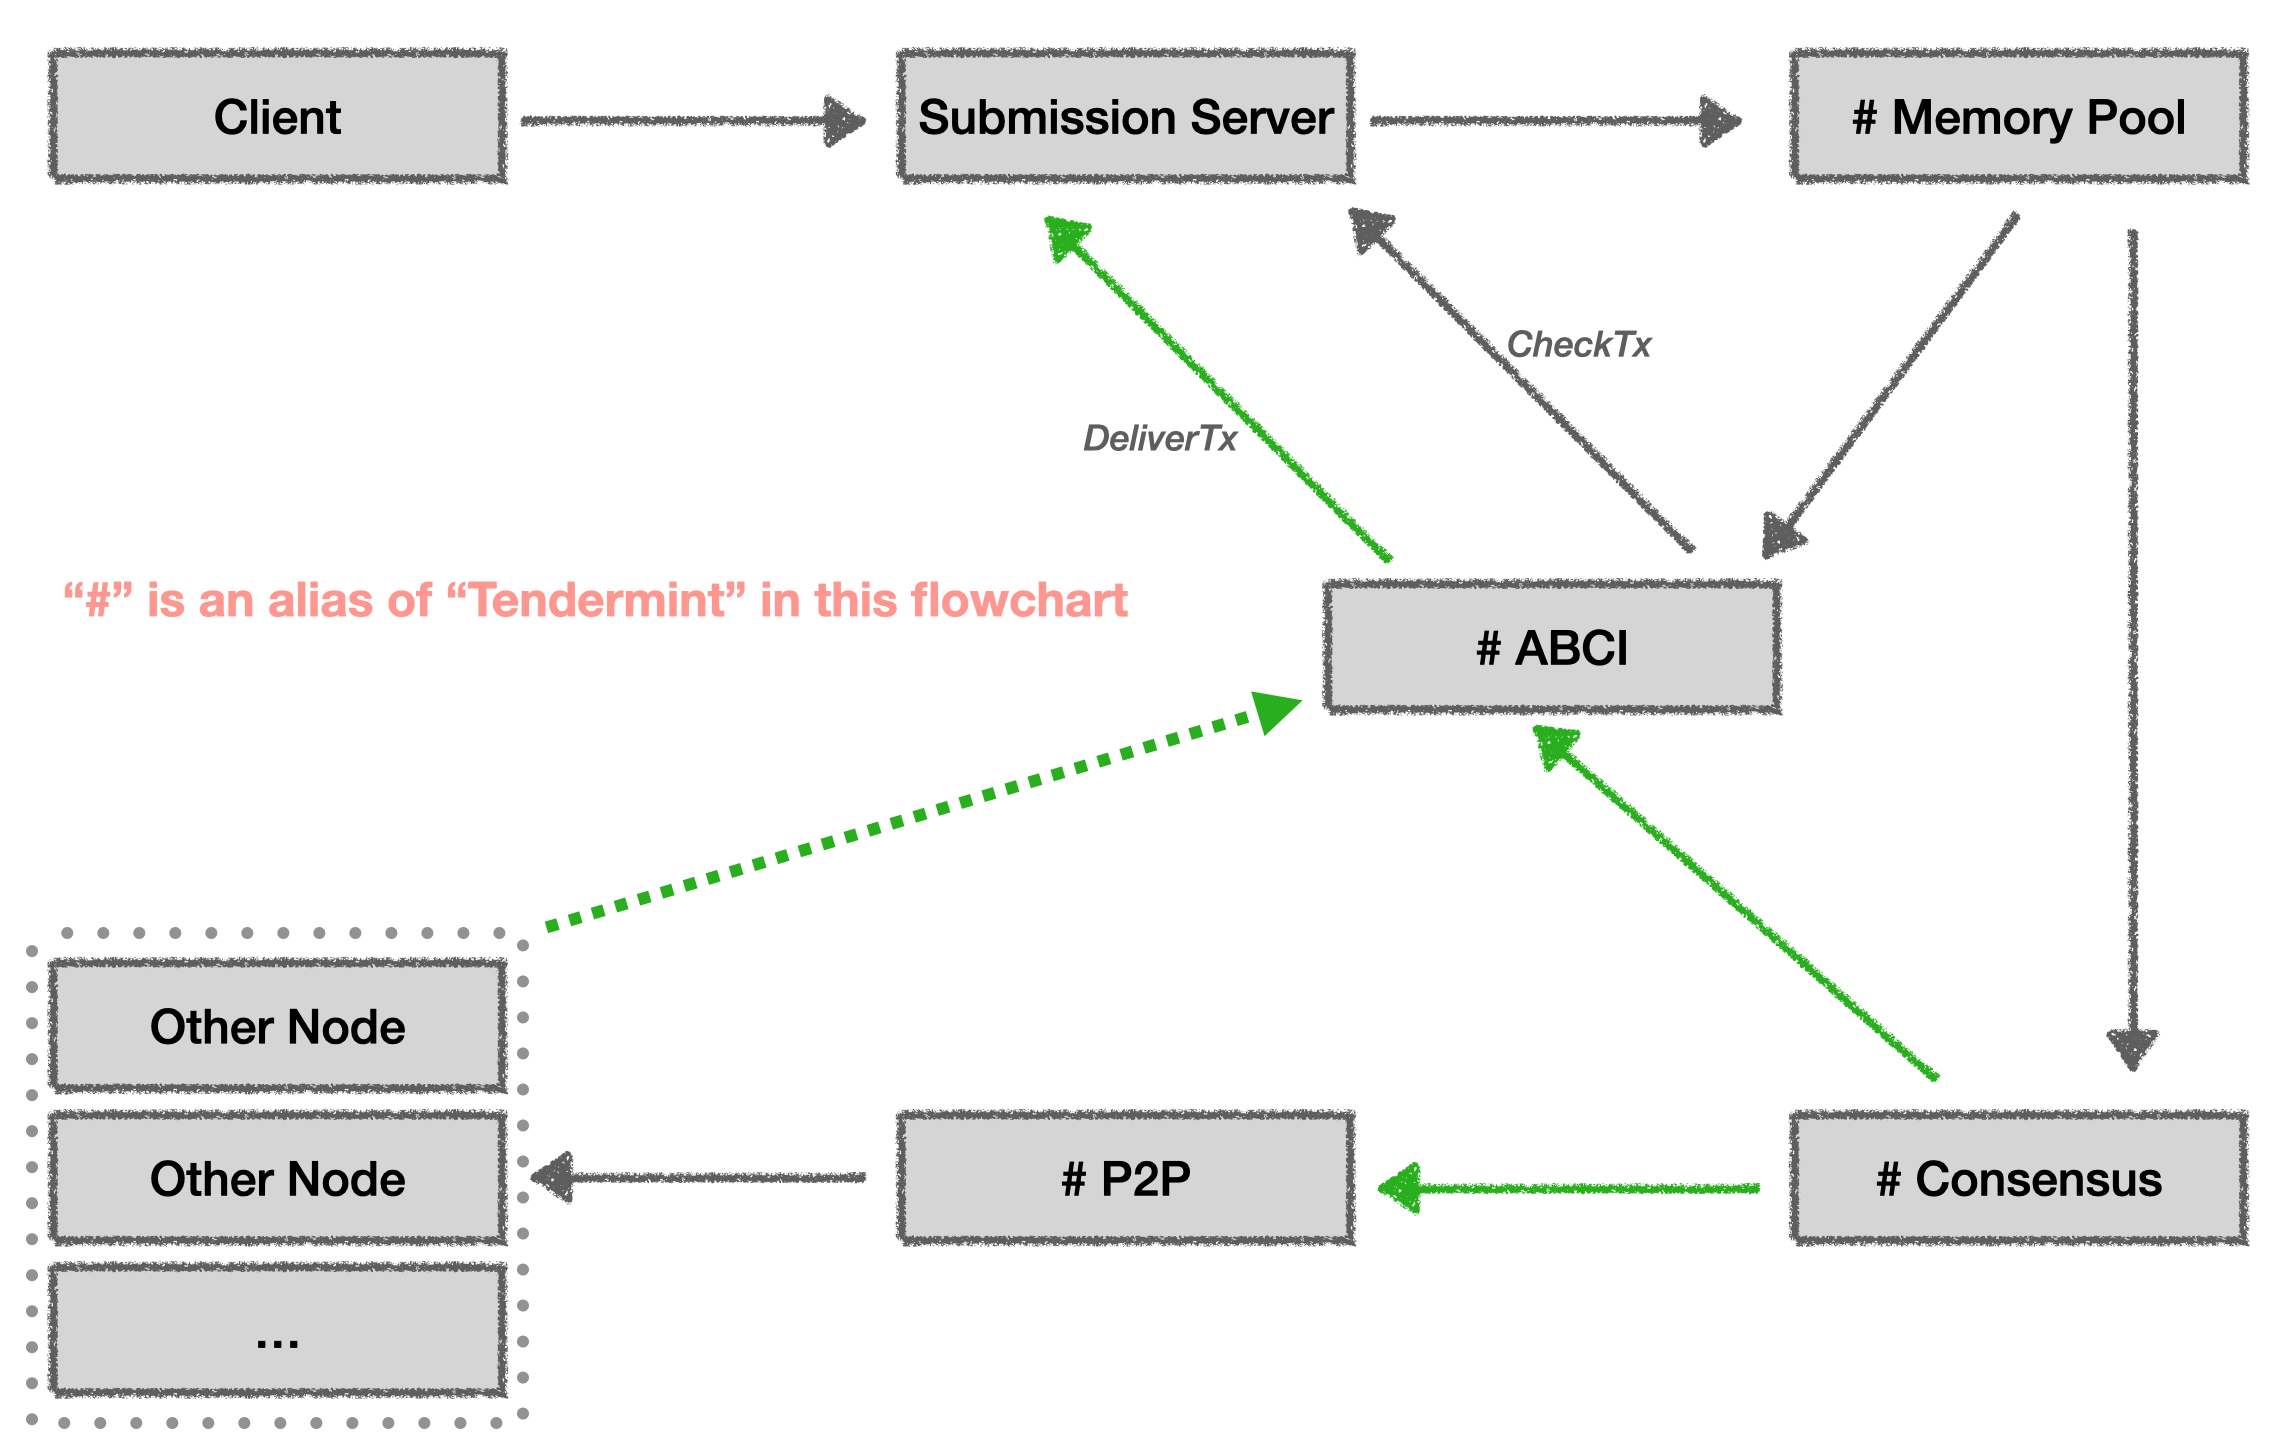
\includegraphics[width=0.9 \textwidth]{/Users/fh/fgr/src/pics/preflow.png}
    \caption{Transactions in Tendermint}
\end{figure}

~\par

Our previous ideas were limited to those blackbox-like operations on the api provided by
\href{https://github.com/tendermint/tendermint}{Tendermint}, this brought many limitations to our action space.
The solutions described in this article no longer use the premise of completely basing on the tendermint API,
and will make changes to the tendermint itself.

The above description may mislead you into thinking that this will lead to more code changes,
but this is not the case, your intuition is wrong.

In fact, this strategy will bring a least damage to the existing code.
When you read the entire content of this article, you will see that
this is almost entirely under the existing framework.
On the contrary, if we don’t make a few changes to ``Tendermint'',
we will be forced to make a lot of ugly changes to our code, which may cause more serious problems.

~\par

Currently, only three parts are covered:

\begin{ITEMIZE}
    \item  transaction fee
    \item  genesis state
    \item  block reward
\end{ITEMIZE}

~\par

More content may be added in the future, the source code of this article is at \href{https://github.com/FindoraNetwork/fgr}{FGR (click here)}.